\documentclass{report}
\usepackage[style=numeric]{biblatex}
\usepackage{multirow}
\usepackage{graphicx}
\usepackage{cleveref}

\addbibresource{references.bib}
\graphicspath{ {../assets/} }

\def\frontmatter{%
    \pagenumbering{roman}
    \setcounter{page}{1}
    \renewcommand{\thesection}{\Roman{section}}
}%

\def\mainmatter{%
    \pagenumbering{arabic}
    \setcounter{page}{1}
    \setcounter{section}{0}
    \renewcommand{\thesection}{\thechapter.\arabic{section}}
}%

\def\backmatter{%
    \setcounter{section}{0}
    \renewcommand{\thesection}{\Alph{section}}
}%
\title{
  Serving AI using a Distributed Architecture \\ 
\begin{large} 
  Final Year Project 2019/20 - Final Report
\end{large} }
\author{Waqas Ali (3035396771)\\\\Supervisor: Dr. Heming Cui\\Mentor: Shixiong Zhao\\\\University of Hong Kong}
\date{\today}
 
\begin{document}

\maketitle

\frontmatter

\addcontentsline{toc}{chapter}{\abstractname}
\begin{abstract}
\thispagestyle{plain}

In recent years, artificial intelligence (AI) has penetrated multiple dimensions of people's daily lives by making the devices they use smarter.
Fueled by data, AI programs imitate human intelligence in terms of their learning and behavioral capabilities.
With such widespread usage, however, users demand improved functionalities and speed, pushing developers and data scientists to make their programs smarter amid industry competition.
These smarter programs have to deal with more complexities, and developers consequently have to choose whether to prioritize the program's features or performance, posing a dilemma for them.
This project proposes to design an AI application with a distributed architecture instead of a centralized architecture (the more common structure in the status quo) to improve its latency, efficiency, and throughput.
As proof of concept, the project specifically examines a complex image analysis service.
The project's objective is to develop tooling and foundation to automatically instantiate and compare distributed systems of a variety of specifications and scheduling algorithms.
There are three milestones in this project.
Firstly, the machine learning stage where test models have to be developed.
Second, modifying the model serving to work in a distributed manner.
Lastly, comparing distributed implementations which is the most crucial aspect of this project.
The project shows that distributed implementations of AI applications lead to better latency, efficiency and throughput.

\end{abstract}

\addcontentsline{toc}{chapter}{Acknowledgements}
\section*{Acknowledgements}
In addition to my supervisor and mentor who helped me with the technical aspects of my project, I would like to thank Ms. Mable Choi (HKU CAES) for her guidance in distilling and consolidating my work in a better way.

\setcounter{page}{2}
\tableofcontents

\newpage
\addcontentsline{toc}{chapter}{\listfigurename}
\listoffigures

\newpage
\addcontentsline{toc}{chapter}{\listtablename}
\listoftables

\newpage
\mainmatter

\chapter{Introduction}

\section{Background}

Artificial intelligence is an area of computer science that focuses on granting machines the ability to act intelligently \cite{McCarthy2007}.
It is a vast field with limitless applications and each application has its own unique solution.
Machine learning, specifically, is a subset of artificial intelligence that learns from data. \cite{Mitchell1997}
Today we see ubiquitous applications of artificial intelligence such as spam filters \cite{Androutsopoulos2000},  recommendations \cite{lekakos2008hybrid}, virtual assistants, and self-driving.

Customers are demanding smarter and smarter capabilities in their machines, and this trend leads to a new set of software development challenges for AI developers. \textit{Nvidia} summarises them with the PLASTER \cite{Teich2018} framework:
\begin{itemize}
  \item Programmability
  \item Latency
  \item Accuracy
  \item Size of Model
  \item Throughput
  \item Energy Efficiency
  \item Rate of Learning
\end{itemize}

These challenges carry over to the realm of machine learning since it is a subset of artificial intelligence.
A machine learning application has two main stages:
\begin{enumerate}
  \item Training (Learning from data)
  \item Inference (Given an input, predicting an output)
\end{enumerate}

Take the example of an application that relies on a machine learning model to transcribe voice.
Before the model can be used by the application, it needs to be trained.
To do this, developers expose the model to hundreds of voice recordings to allow it to learn which sounds match to which words.
Now, the application can use the model by sending it voice recordings and receiving transcribed text in return.
In short, this process of predicting an output in response to an unseen input is inference, the second stage of machine learning as mentioned previously.

\section{Motivation}\label{motivation}

\begin{figure}
  \centering
  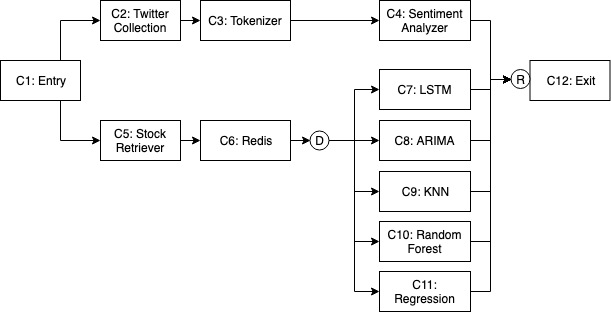
\includegraphics[width=\textwidth]{StockPriceServiceBasic.png}
  \caption{Inference pipeline of a stock price prediction service. C2 and C5 are data retrievers that fetch past stock data and twitter mentions of a specified stock symbol. C6 is a caching layer that allows skipping C7-C11 steps if a prediction has been recently made for a specific stock symbol. C7, C8, C9, C10 \& C11 are ML models that compete against each other to predict a stock symbol's price. C4 is a sentiment analyzer whose results are taken into account for price prediction. As can be seen, it is a fairly complex pipeline composed of several different steps.}
  \label{fig:StockPriceServiceBasic}
\end{figure}

Since end-users of machine learning applications are only concerned with inference, not training, the inference must be quick.

For inference, an input goes through multiple steps, known as a pipeline.
Figure \ref{fig:StockPriceServiceBasic} is an example of a stock price prediction service's pipeline.
As tasks in a pipeline increase in quantity and complexity, it can increase the \textit{latency} (time taken) to execute all steps of the pipeline.
Moreover, if a \textit{centralized architecture} (single machine) executes the complete pipeline, it can create bottlenecks.
For example, if a pipeline for input A is in progress, the pipeline for input B cannot start.

On a centralized architecture, all tasks have to be done sequentially (even if they are independent of each other).
This could take a long time and hence increase the \textit{latency}.

Consequently, it is also possible for hardware resources to go underutilized and used for longer periods leading to decreased \textit{efficiency}.

Moreover, until all tasks for a specific request have finished, processing for a new request cannot start.
Thus, the service cannot handle a high number of requests in a given period i.e. \textit{throughput}.

\section{Objectives}\label{objectives}

Several methods could be considered to optimize latency, throughput, and efficiency of artificial intelligence applications.
This project tackles this optimization problem by efficiently distributing the pipeline tasks of artificial intelligence applications over several machines.

Moving an artificial intelligence application from a centralized architecture to a distributed architecture not only requires deploying it on a network of multiple machines but modifying it to properly utilize the newly available resources.

A distributed application's success depends on how the application divides its tasks (job scheduling) and the quality/quantity of resources available for use.
To figure out what works best we need a quick and reliable way of testing different job scheduling algorithms on networks of different sizes composed of machines of different specifications.

Consequently, the project's objectives are to develop the following programs:
\begin{enumerate}
  \item An AI application with a complex inference pipeline that can work with different job scheduling algorithms.
  \item A deployment method that can programmatically deploy an AI application according to provided specifications.
  \item A web app to measure latency, efficiency and throughput in an architecture-agnostic way.
\end{enumerate}

With the above-mentioned programs in place, we can confidently investigate and argue for or against using distributed systems for AI applications.

\section{Contribution}\label{contribution}

With data, the project shows that latency, efficiency, and throughput of an AI application (concerns which were highlighted in the PLASTER framework \cite{Teich2018}) can indeed be improved if a decentralized architecture is employed instead of a centralized architecture.
Moreover, the project contributes tools to better conduct similar investigations.

\section{Report Organization}

Composed of artificial intelligence, distributed systems, and web development, the project's methodology involves several fields of computer science and software engineering to achieve the objectives mentioned in section \ref{objectives}.
Naturally, that invites its own set of complexities and uncertainties. 
After literature review and project reasoning in \cref{litreview}, \cref{chap:methodology} accomplishes the important task of narrowing down and justifying the methodology.
Following this, \cref{chap:implementation} discusses in detail the implementation and technical details of the project.
Most importantly, \cref{chap:results} shows the results.
Lastly, \cref{chap:conclusion} summarises this report and the project.

\chapter{Literature Review and Justification}\label{litreview}

\section{Literature Review}

Published in 2011, Mesos \cite{Mesos} was a pioneering work in resource-sharing across cluster-computing frameworks.
It introduced a two-level scheduling mechanism that resulted in near-optimal performance and reduced resource under-utilization.

In 2017, Clipper \cite{Clipper} was introduced as a general-purpose prediction system that acted as a model selection/abstraction layer between applications and different implementations of a model.
This ultimately allowed an AI model to be easily deployed on a distributed system while gaining benefits of modular architecture and increased performance.

Coming from the same lab as Clipper \cite{Clipper}, InferLine \cite{InferLine}, published in 2018, was a general-purpose specification designed to proactively optimize ML inference pipelines but also reactively control configurations. While generalizing across different frameworks, it achieved 7.6 times cost-savings and 32 times lower SLO miss-rate.

Lastly, GrandSLAm \cite{GrandSLAm}, published in 2019, was a general-purpose framework to optimize clusters serving multiple microservice-based applications.
It increased the throughput of pipelines by three times without sacrificing on latency by batching requests to common microservices.

\section{Shortcomings}

Mesos \cite{Mesos} is great at resource-optimization but it does not take into account the bigger picture.
It is only concerned with how much resources the task at hand requires.
Hence, it is not suitable for complex machine learning pipelines such as the one in figure \ref{fig:StockPriceServiceBasic}.

Clipper \cite{Clipper} deals with different implementations of the same model. In the case where we have different models in a pipeline, we lose out on its benefits.

GrandSLAm \cite{GrandSLAm} is for scenarios where multiple pipelines have tasks i.e. microservices in common. As it is focused on optimizing microservice execution, it is different from our objectives.

InferLine \cite{InferLine} is an interesting approach to solving the problems highlighted in section \ref{motivation}.
However, a public implementation is unavailable and hence further work cannot be done on it to improve it.

\section{Project Justification}

Regardless of how the pipeline optimization problem is solved, an implementation-agnostic way is needed to measure the results.
In addition to its approach to solving the problem, this project also develops tools that can be used in the future to easily deploy and compare other solutions.
Moreover, it builds a foundation, utilizing available resources at the University of Hong Kong, on which further work can be carried out.

\chapter{Methodology}\label{chap:methodology}

From developing an artificial intelligence application to running it on a distributed architecture to comparing it to a traditional implementation, there are many steps to this project and without proper breakdown, it could get overwhelming quickly.
The following sections describe and justify the steps through which the project aims to accomplish its objectives.

\section{Choose AI Application for testing}

\begin{figure}[h!]
  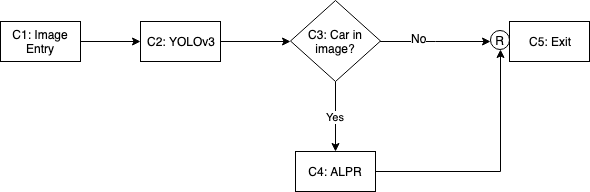
\includegraphics[width=\textwidth]{CurrentImageService.png}
  \caption{Inference pipeline of an image analysis service. It starts with C1 where an image is given as input. C2 runs the image through YOLOv3 \cite{YOLOv3} to detect the objects in it. C3 is a conditional where it checks if there is a car in the image. If true, the image goes through ALPR \cite{OpenALPR} to extract the nameplate details. The pipeline ends at C5 by returning the detected objects and nameplates in the image. With multiple models and branching, the pipeline represents real-world services e.g. Facebook image moderation, Google image labeling, etc.}
  \label{fig:CurrentImageService}
\end{figure}

As the project proposes a distributed architecture for artificial intelligence applications, our test AI application must be a sufficient representative of most if not all AI applications for a fair investigation.
Naturally, a fairly representative application is one with a pipeline composed of different kinds of tasks with a mix of mutually dependent and independent ones.
Ergo, choosing a single AI application as a testing ground for our solution is an important task that requires studying popular AI techniques and implementations in the community.

\section{Develop basic application}
For any artificial intelligence application, first of all, machine learning models need to be trained and an inference pipeline needs to be developed.
This requires studying current techniques for the application of our choice and using that knowledge to build and train good enough models.
At this stage, accuracy is not important so we do not need to fine-tune the models.
Once the model training is done, it needs to be ready for inference.
Therefore, we need to ensure that all the steps required to accomplish inference on unseen inputs have been implemented at a satisfactory level.

\section{Run on a centralized system}
After having chosen a test AI application and trained basic models for it, we need to ensure we can successfully run inference on a single machine.
This step is important for two reasons.
Firstly, this gives us a baseline performance we can compare our distributed implementations with.
Second, we will have a working implementation of our application and we can refer to it while converting our application to work with a distributed implementation.

\section{Convert to a distributed system}
Consequently, the next step is to convert the application from a centralized implementation to a distributed implementation.
This will require modifying the source code to use distributed system techniques such as RPC (remote procedure call).
To ensure consistency, we should ensure our distributed implementation running on one machine has the same performance as the centralized implementation from earlier.

\section{Programmatic Deployment}
The only way to test a distributed implementation is to deploy it on a cluster of computers and measure performance.
We also need to vary the cluster specifications and test repeatedly.
Moreover, we need to ensure all specifications are reproducible and give consistent performance.
Doing all this manually can get complex and out of control quickly.
Therefore, having a programmatic way of deploying and keeping track of distributed system deployments is crucial.

\section{Compare architecture-agnostically}
With all these different deployments, we need a reliable way of comparing each deployment performance that is completely decoupled from its intrinsic qualities.
A fair and reliable way to compare is to create a web app that accepts a server URL and sends numerous requests to it.
As the web app is run in the browser, it measures these metrics from the client-side and all it cares about is input and output.
Thus, it does not matter for the web app if the server implementation is on a centralized or distributed architecture.

\subsection{Test Cases}
To study whether a distributed architecture can indeed improve latency, efficiency, and throughput, performance will be compared across systems of various specifications:

\begin{enumerate}
  \item Centralized implementation (baseline)
  \item 1 machine for n tasks (should be same as above)
  \item Less than n machines for n tasks
  \item n machines for n tasks (optimum)
\end{enumerate}

\section{Summary}
To summarise, the project picks an AI application, builds it to run on a centralized architecture, converts the application to run on a distributed architecture, runs the application on distributed systems of different specifications and, lastly, compares the application across all these implementations to assess whether latency, efficiency, and throughput can be improved using a distributed architecture.

\chapter{Implementation}\label{chap:implementation}

The next few sections highlight the implementation of the methodology discussed in \cref{chap:methodology}.
It incorporates state-of-the-art open-source technologies and reproducible techniques while adapting to resource constraints.

\section{AI Application of Choice}

\begin{figure}[h!]
  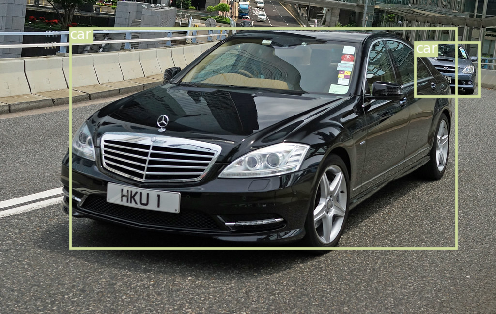
\includegraphics[width=\textwidth]{hku1.jpeg}
  \caption{YOLOv3 Results. It shows two correctly identified cars and their location in image.}
  \label{fig:YOLOResults}
\end{figure}

An image analysis service (Figure \ref{fig:CurrentImageService}) was chosen for multiple reasons.
First of all, image services are quite common nowadays and thus representative of the production landscape of artificial intelligence.
Second, there are several open-source models e.g. YOLOv3 \cite{YOLOv3} available so we can save time by not developing our own.
Moreover, we can replicate real-world load by using them.
Lastly, GPUs are fundamental to machine learning and our experiments need to take their usage into account.
As image models heavily rely on GPUs, they are perfect candidates for being part of our inference pipeline.

\section{Architecture (Simplified)}

\begin{figure}[h!]
  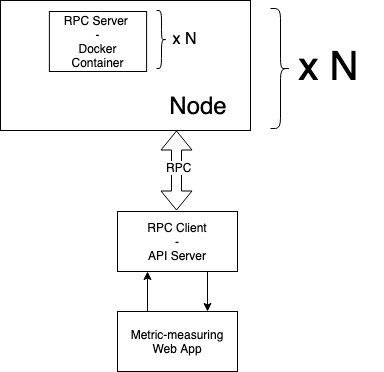
\includegraphics[width=\textwidth]{Infrastructure.png}
  \caption{Project Architecture. A web app interacts with an API server which fulfills requests by communicating using RPC with pipeline task instances deployed across several machines.}
  \label{fig:Infrastructure}
\end{figure}

As figure \ref{fig:Infrastructure} shows, the application architecture involves remote procedure calls to instances of pipeline tasks running across multiple machines.

\subsection{Container for each pipeline task.}

\begin{figure}[h!]
  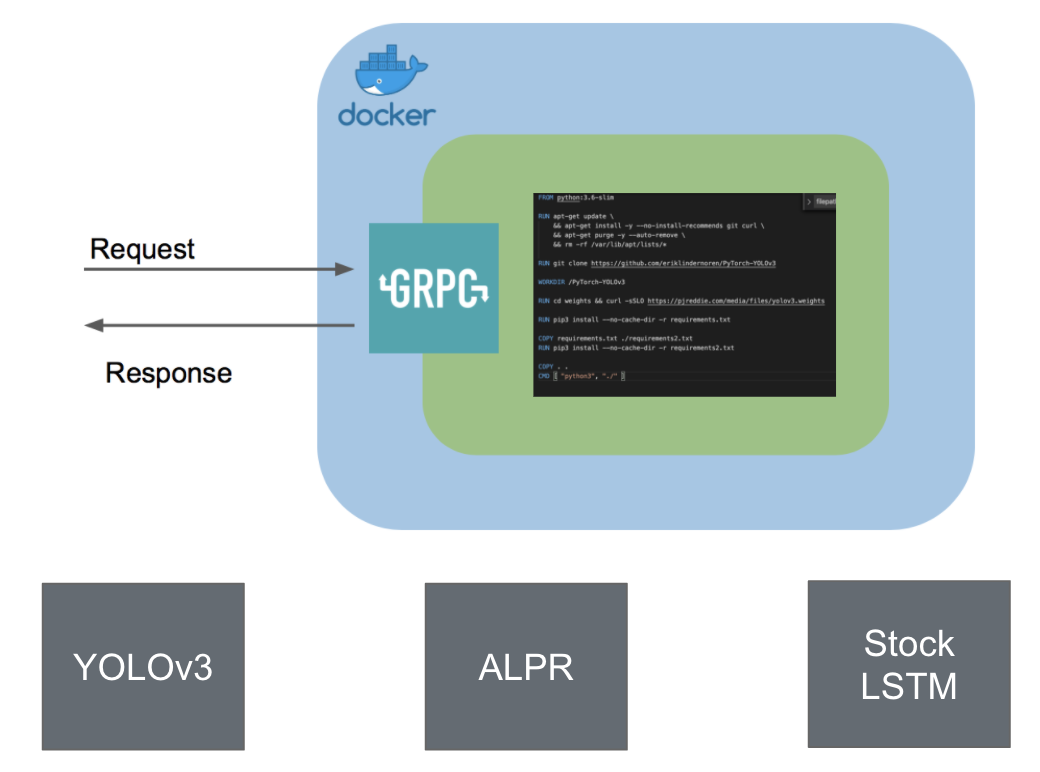
\includegraphics[width=\textwidth]{docker.png}
  \caption{Containerization using Docker. Docker has been used to run isolated gRPC server containers for each task of the pipeline.}
  \label{fig:YOLOResults}
\end{figure}

Docker \cite{Docker} has been used to run separate \textit{containers} for each task of our pipeline e.g. YOLOv3.
This makes it easy to develop, package, and deploy each task reliably.
As long as we have Docker running on our cluster nodes, we can run any task on any node.
If OpenALPR requires a specific version of Linux but YOLOv3 requires something else, we don't have to worry about finding common ground.
Using Docker, we can isolate each task into its runtime and start/stop/restart it at any time.
Moreover, we can scale up or down the number of tasks with just a single instruction.

\subsection{Remote Procedure Calls}

For remote procedure calls, gRPC \cite{gRPC} is used because it is open-source, modern (uses HTTP/2), efficient and cross-platform (uses Protocol Buffers as the interface description language).
To implement gRPC, every \textit{task container} of the pipeline is a gRPC server.
Our API server acts as a gRPC client when communicating with any task instance.
Because gRPC is cross-platform, we are not limited by our choice of language/framework to build our RPC servers.
All we need is to define our task as a gRPC service using \textit{Protocol Buffers} \cite{ProtocolBuffers} (a method of serializing structured data).

\subsection{API Server}

Our API server is the bridge between our client and our task instances.
It implements the \textit{REST} architecture style using \textit{Python} and \textit{Flask}.
As it is responsible for managing our task instances, all the \textit{scheduling} logic lies here.
By changing how it fulfills the requirements of incoming requests, we can increase/decrease the performance of our distributed system.

In addition to accepting inputs for our image analysis pipeline, it also accepts inputs to the scheduling logic.
This allows us to easily modify its behavior while conducting experiments.

\subsection{Web App}

\begin{figure}[h!]
  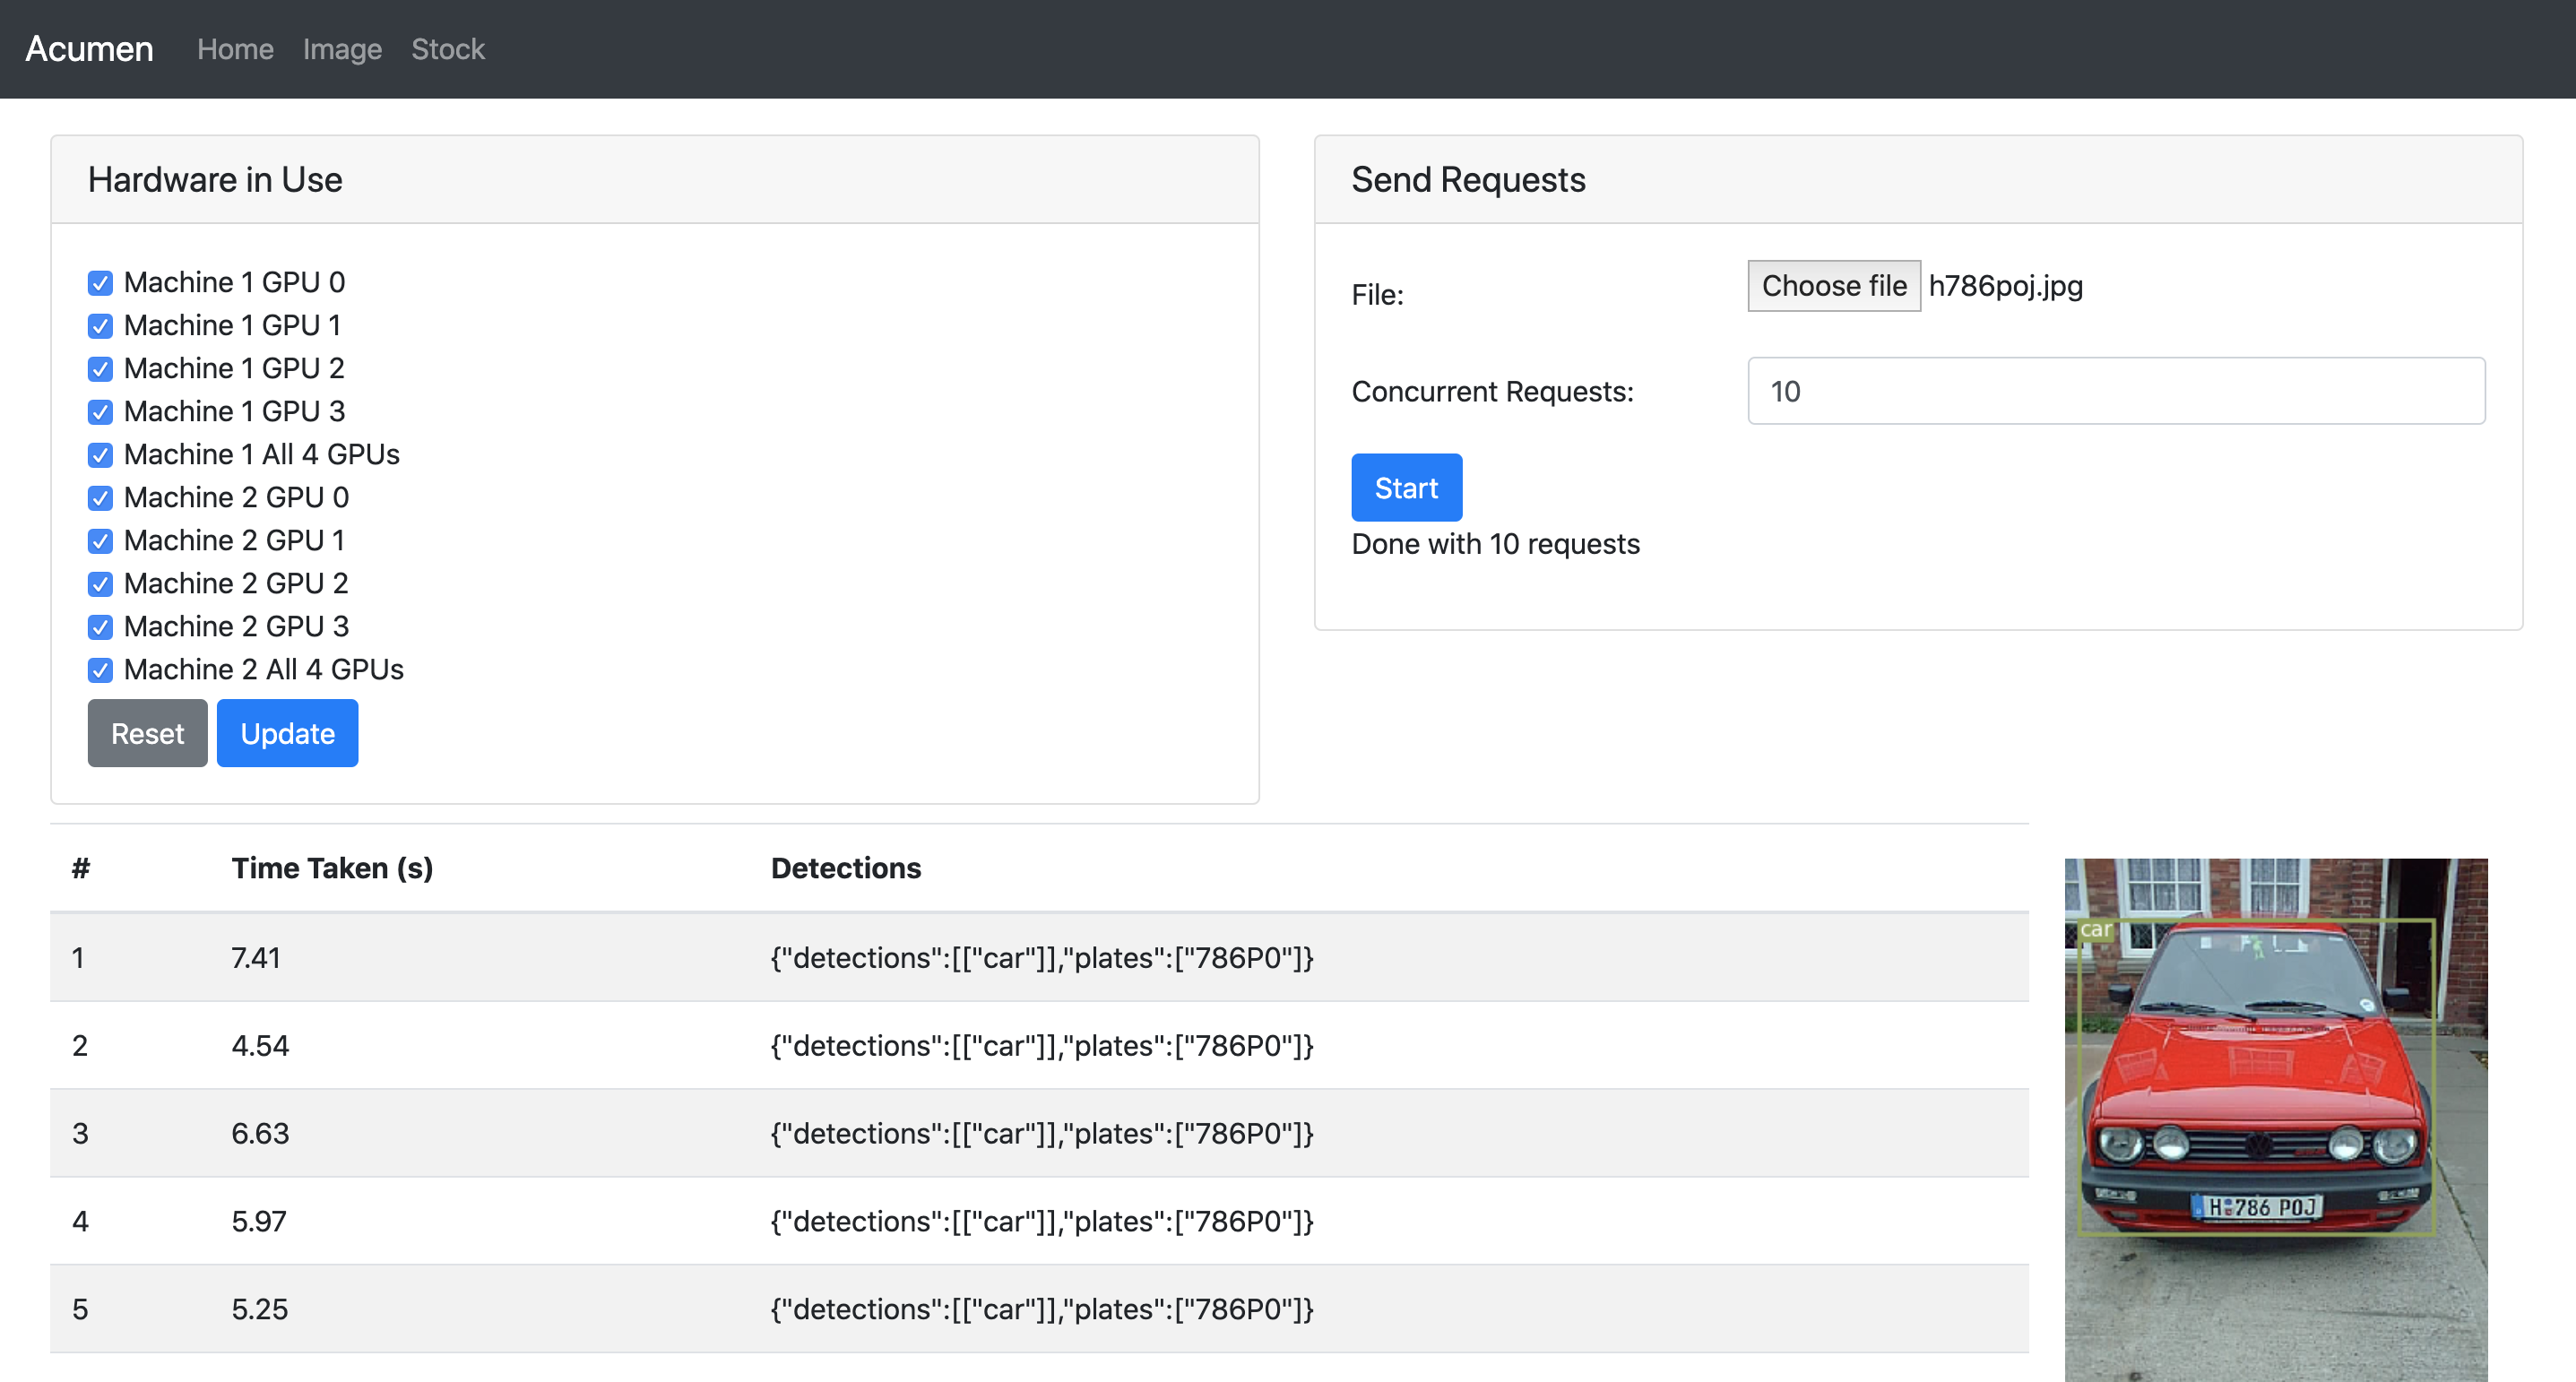
\includegraphics[width=\textwidth]{acumenwebapp.png}
  \caption{Metric-measuring Web App. The distributed system's specifications can be modified using the "Hardware In Use" panel on top left. The "Send Requests" panel on the right is used to control the number of concurrent requests. The results section shows the output and response time for each request.}
  \label{fig:WebApp}
\end{figure}

The purpose of the web app is three-fold.
First, we can use it to send requests and measure response time.
Second, we can modify the type/number of requests we send.
Third, we can set the scheduling logic of the API server.
With these three functions, we can conduct all kinds of experiments and collect valuable data for our project.

The web app is a fully client-side and all the required \textit{HTML}, \textit{CSS} and \textit{JavaScript} is fetched once in the beginning.
This ensures our API server is not wasting valuable resources rendering web pages.
It is built using \textit{JavaScript} and \textit{React}.
As it does not know how the API server works other than the kind of input it accepts and the output it sends back, our web app is fully architecture-agnostic.

\section{Architecture (Actual)}

As with any real-world implementation, we are constrained by the resources we have at hand. To overcome them, the architecture has been slightly modified as shown in figure \ref{fig:InfrastructureDepartment}.

\begin{figure}[h!]
  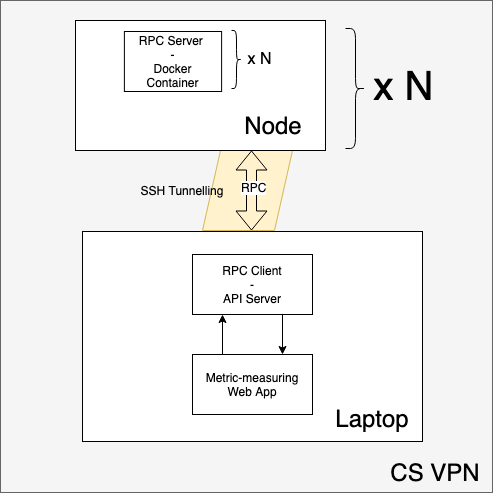
\includegraphics[width=\textwidth]{InfrastructureDepartment.png}
  \caption{Modified architecture to overcome resource constraints. SSH tunneling has been used to port forward API server's ports to task instances. The entire architecture runs on the CS VPN.}
  \label{fig:InfrastructureDepartment}
\end{figure}

\subsection{Challenges}

The machines available for use at the Computer Science department of the University of Hong Kong have highly powered CPUs (Intel(R) Xeon(R) Silver 4116 CPU @ 2.10GHz) and GPUs (4 x GeForce RTX 2080 Ti). However, using them involved a few challenges:
\begin{enumerate}
  \item All ports are blocked
  \item Only SSH is allowed
  \item CSVPN is required
\end{enumerate}

As RPC communication between our API server and the task instances running on these machines requires several ports to be open, it was a make-or-break situation. But on the other hand, it would have been costly not to use these machines so overcoming these challenges was important.

\subsection{CS VPN}

The first solution was to use the same machine to run the API server and browse the web app.
If connected to CS VPN, the machine allows us to communicate with other department machines via SSH.

\subsection{SSH Tunneling}

\begin{figure}[h!]
  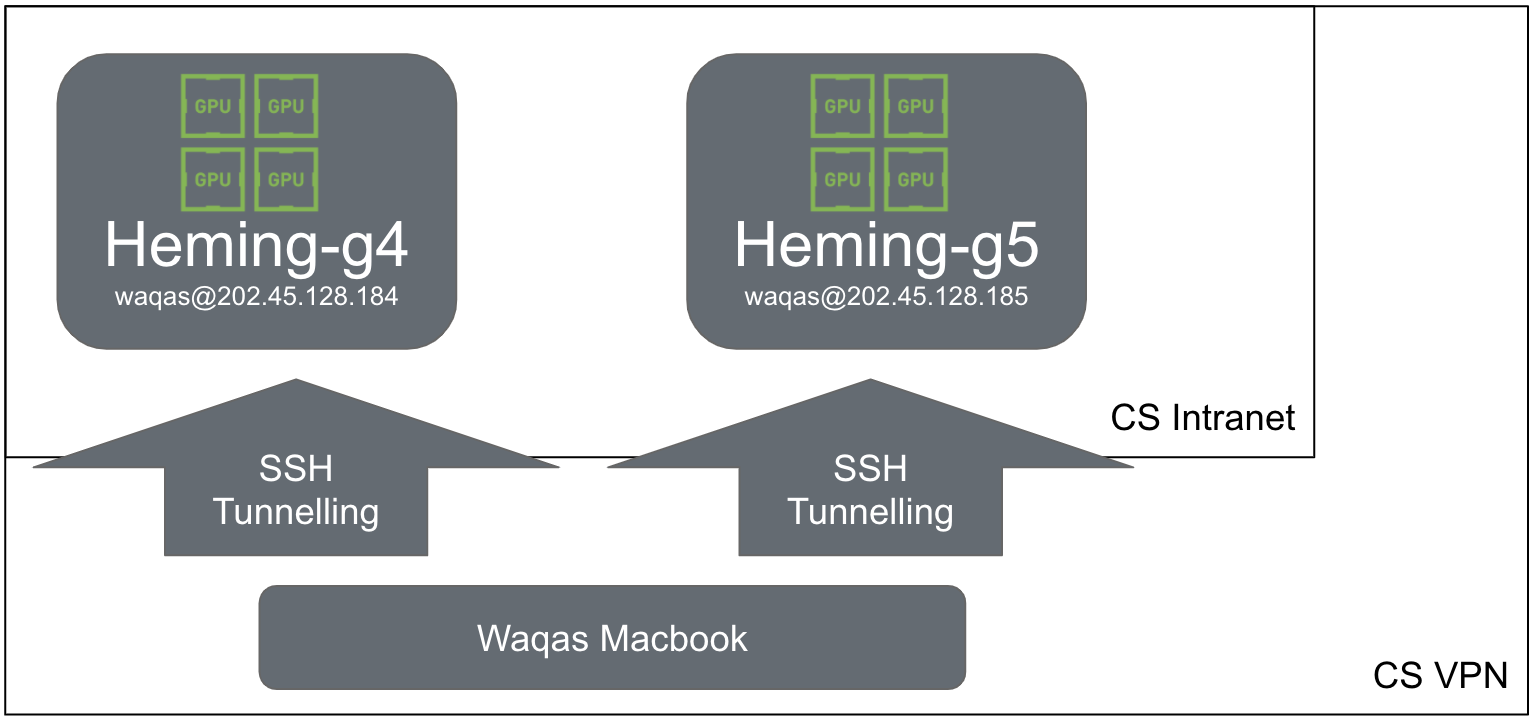
\includegraphics[width=\textwidth]{sshtunneling.png}
  \caption{SSH Tunneling to connect to task instances from my Macbook running the API server.}
  \label{fig:sshtunneling}
\end{figure}

Because all ports are blocked on department machines except SSH (22), SSH tunneling was used for port forwarding (Figure \ref{fig:sshtunneling}).
What that means is that the API server acts as if the task instances are running on the same machine as itself but the port requests are forwarded to cluster machines via SSH tunneling.

\section{Deployment \& Source Code}

\section{Terraform}

\begin{figure}[h!]
  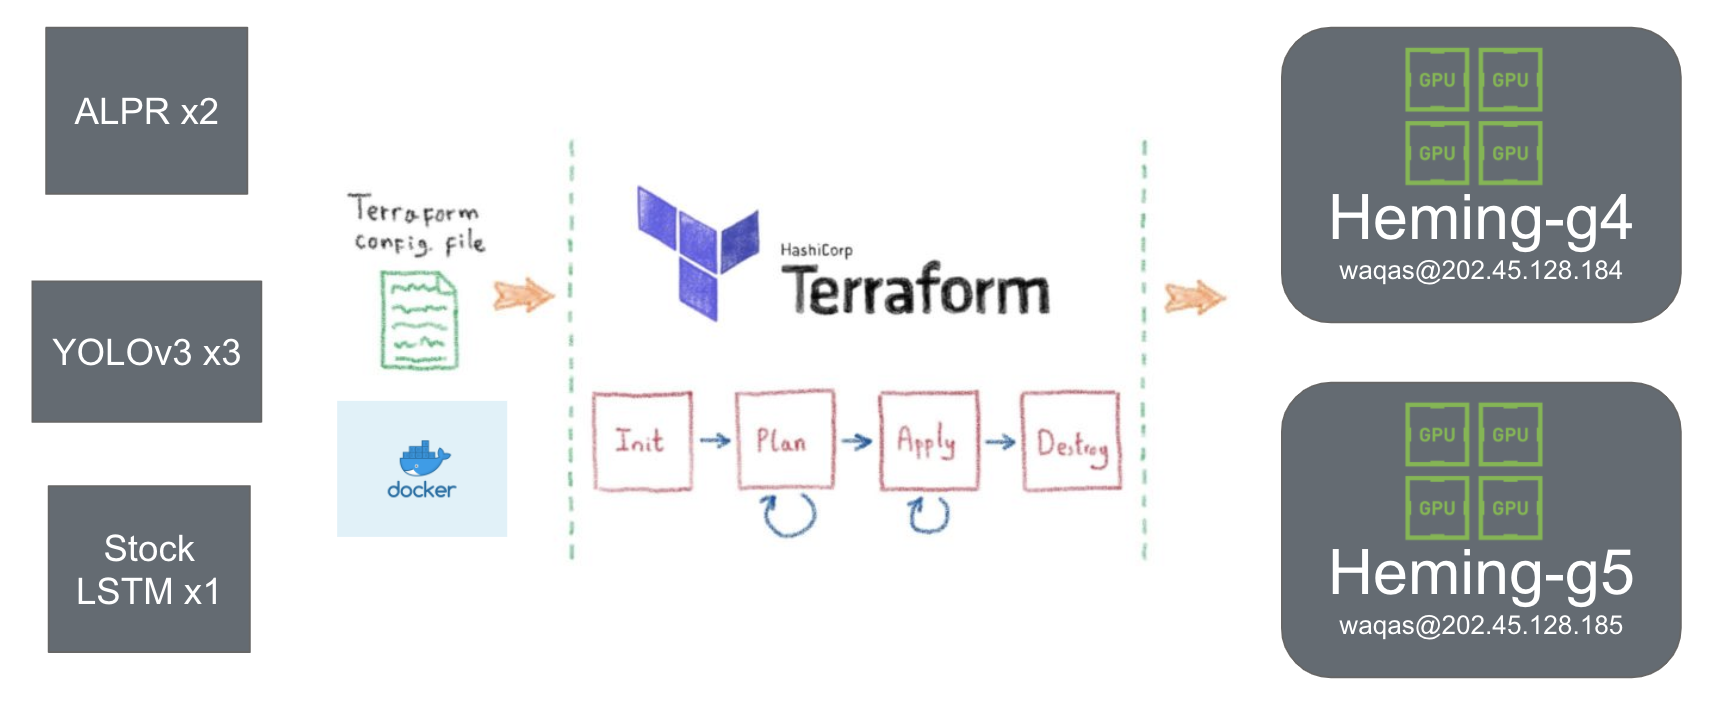
\includegraphics[width=\textwidth]{terraform.png}
  \caption{Deployment using Terraform. By writing our infrastructure as code in config files, we can easily track, manage, scale and deploy our experiments.}
  \label{fig:Terraform}
\end{figure}

With complex pipelines, several machines and tens of task instances, it is highly important to track deployment.
Through \textit{Terraform} \cite{Terraform}, we can programmatically deploy and manage our infrastructure.
If we need to increase or decrease the number of YOLOv3 instances across multiple machines (while keeping track of their port numbers), we only need to modify a single config file, and Terraform handles the rest.
Moreover, this brings infrastructure under version control, allows reproducibility and increases scalibility (more machines can be easily added).

\section{Source code}

To ensure the project is replicable and open to further improvement, the source code has been made available. \cite{SourceCode}
With the tools the project publishes, it hopes to contribute to further research in distributed systems at the University of Hong Kong.

\chapter{Results}\label{chap:results}

\begin{table}[h!]
  \begin{center}
    \caption{Response times for Image Analysis pipeline with a car image as input. n represents the number of concurrent requests. Each column represents the number of task instances in the distributed system. n/2 for n in the case of n = 10 means that there were 5 instances each of YOLOv3 and OpenALPR available for use. The response time is the total time it took for all requests to finish (averaged over three trials)}
    \label{tab:results}
    \begin{tabular}{|l|l|l|l|}
      \hline
      Requests (n) / Task instances & 1 for n (baseline) & n/2 for n & n for n (optimum) \\ \hline
      1                                                 & 4.61s      & 4.60s        & 4.64s      \\ \hline
      10                                                & 46.41s      & 9.30s        & 4.59s      \\ \hline
      50                                               & 231.22s      & 9.29s        & 4.61s     \\ \hline
      \end{tabular}
  \end{center}
\end{table}

\chapter{Conclusion}\label{chap:conclusion}
The project has three crucial parts: machine learning, tooling, and distributed architecture.
As shown in \cref{chap:implementation}, a functional image analysis service has been developed and deployed which closely resembles machine learning applications in the real world.
Moreover, reliable tooling has been successfully developed for metric measurement and deployment that can be used outside of this project.
Adding to that, a distributed implementation has been developed.
As mentioned in \cref{chap:methodology}, the hypothesis mentioned in section \ref{contribution} (distributed architecture is better than traditional architecture) has been tested using a production-representative machine learning application and reliable metric tooling.
With the data obtained from these tests (Table \ref{tab:results}), the project has shown that the latency, efficiency, and throughput of AI applications can be improved using a distributed architecture.

\backmatter

\addcontentsline{toc}{chapter}{Bibliography}
\printbibliography

\end{document}